\section{Making a change}
\begin{frame}[fragile]
  \slidetitle

  This section covers the following topics:
  \begin{itemize}
    \pause
    \item See the commit history
    \pause
    \item Make commits that are actually changes
    \pause
    \item Change commits and the history
  \end{itemize}
\end{frame}

\subsection{Commit logs}
\begin{frame}[fragile]
  \subslidetitle

  The command \cmd{git log} displays the commit history:
  \begin{lstlisting}
$ (*\textcolor[HTML]{0000AA}{git log}*)
(*\textcolor[HTML]{ae6617}{commit 633a534830c18a1747aaa5677aa6ec0b18f250c4}*)
Author: Andr(*é*) Roth <neolynx@gmail.com>
Date:   Sat Nov 21 13:51:18 2015 +0100

    green moon

(*\textcolor[HTML]{ae6617}{commit 368a328bbefccbdf5732ca90b95015061186e16a}*)
Author: Andr(*é*) Roth <neolynx@gmail.com>
Date:   Sat Nov 21 13:47:14 2015 +0100

    title in page

...
\end{lstlisting}
Note: \cmd{git log} uses a pager to display the log, use \cmd{q} to quit.
\end{frame}

\subsection{Commit logs on one line}
\begin{frame}[fragile]
  \subslidetitle

  In our commit history we find the following messages:
  \begin{lstlisting}
$ (*\textcolor[HTML]{0000AA}{git log --oneline}*)
(*\textcolor[HTML]{ae6617}{633a534}*) green moon
(*\textcolor[HTML]{ae6617}{368a328}*) title in page
(*\textcolor[HTML]{ae6617}{96c4f6a}*) blue moon
(*\textcolor[HTML]{ae6617}{5784ef6}*) we do not need the test file anymore
(*\textcolor[HTML]{ae6617}{13dbd70}*) adding test file
(*\textcolor[HTML]{ae6617}{3ce2637}*) change title
(*\textcolor[HTML]{ae6617}{220767d}*) add authors file
(*\textcolor[HTML]{ae6617}{39719c9}*) initial commit
\end{lstlisting}
\end{frame}

\subsection{Showing a commit detail}
\begin{frame}[fragile]
  \subslidetitle
The \cmd{git show} command gives details about a specific commit hash.

\begin{lstlisting}
(*\textcolor[HTML]{0000AA}{git show 220767d}*)
(*\textcolor[HTML]{B7A000}{commit 220767dbb3ab047e548752b744699731e1c38509}*)
Author: Andr(*é*) Roth <neolynx@gmail.com>
Date:   Mon Nov 9 21:44:02 2015 +0100

    add authors file

diff --git a/AUTHORS b/AUTHORS
new file mode 100644
index 0000000..8227a64
--- /dev/null
+++ b/AUTHORS
(*\textcolor[HTML]{18B2B2}{@@ -0,0 +1 @@}*)
(*\textcolor[HTML]{00AA00}{+Tux Penguin}*)
\end{lstlisting}

Note: the hashes can be abbreviated to their short form (\cmd{220767d})
\end{frame}

\subsection{Textmode Interface for git - tig}
\begin{frame}[fragile]
  \subslidetitle
  The program \cmd{tig} displays the history and allows to control git interactively:
  \newline \vspace{1em}
  \centerline{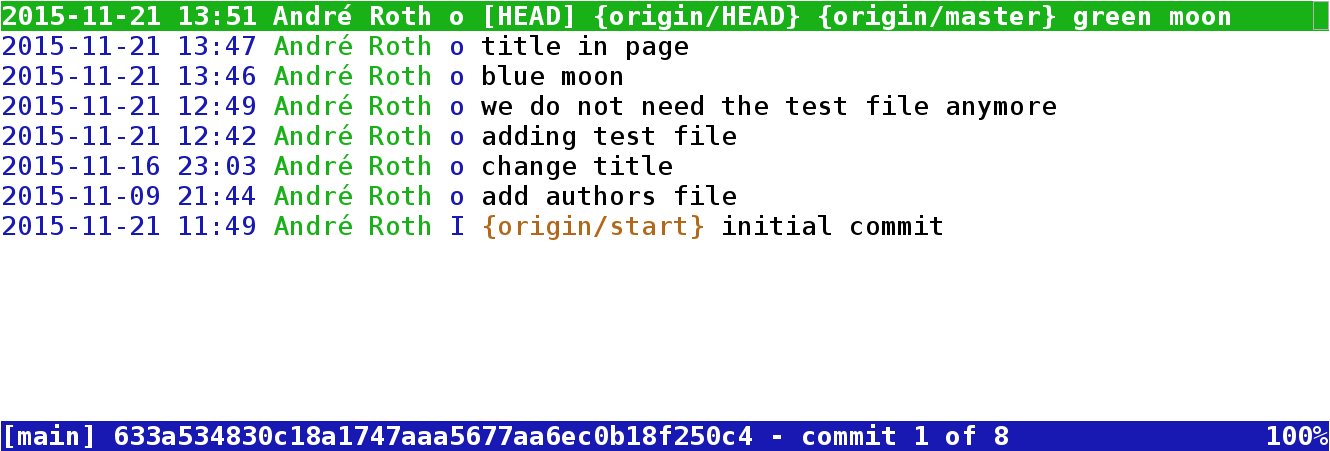
\includegraphics[width=10.5cm]{../screen/tig_screenshot.png}}

  \vspace{1em}
  Note: Press \cmd{q} to quit, or \cmd{h} for help.
\end{frame}

\subsection{gitk}
\begin{frame}[fragile]
  \subslidetitle
  The program \cmd{gitk} allows to display and control git commits in a GUI:
  \\
  \vspace{1em}
  \centerline{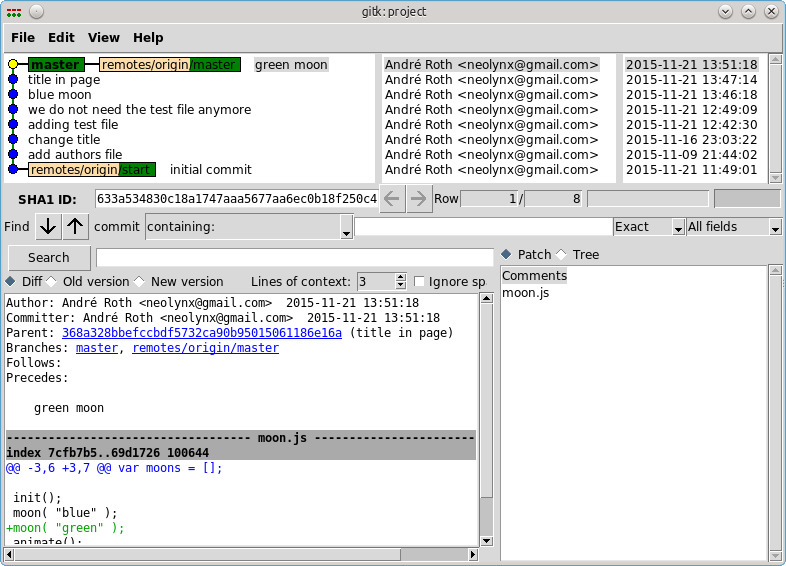
\includegraphics[width=9cm]{../screen/gitk.png}}
\end{frame}

\subsection{Git commits}
\begin{frame}[fragile]
  \subslidetitle
  Using git correctly means a commit is not just a saved snapshot of your ongoing work. \\
  \vspace{1em}
  \textbf{A commit is a change to the software.} \\
  \vspace{1em}
  Best practices for git commits:
  \begin{itemize}
    \item Use the imperative mood in the subject line \\
      'add file', not 'adding file' or 'added file'
    \item A git commit contains only the diffs that are needed for that given change
    \item shows whether a developer is a good collaborator.
    \item Limit the subject line to 50, wrap the body at 72 characters
    \item Use the body to explain What and Why vs. How
  \end{itemize}
\end{frame}

\subsection{Git commits}
\begin{frame}[fragile]
  \subslidetitle

  A git commit consists of the following elements:
  \begin{tabular}{lp{10cm}}
    \pause
    \textbf{Message Title} & A title describing the change \\
    \pause
    \textbf{Message Body} & A message body explaining the change \\
    \pause
    \textbf{Author} & Name and Email of author \\
    \pause
    \textbf{Author Date} & Date of commit \\
    \pause
    \textbf{Committer} & Name and Email of committer \\
    \pause
    \textbf{CommitDate} & Date of commit \\
    \pause
    \textbf{SHA} & HASH which git uses as key \\
  \end{tabular}

  \vspace{1em}
  Note: Your commit message reveals whether you are a good collaborator or not.
\end{frame}

\subsection{Interactive rebase}
\begin{frame}[fragile]
  \subslidetitle

  Let's revisit the last 6 commits:
  \begin{lstlisting}
$ (*\textcolor[HTML]{0000AA}{git rebase -i HEAD\textasciitilde6}*)
(*\textcolor[HTML]{B7A000}{pick}*) (*\textcolor[HTML]{349E9E}{3ce2637}*) (*\textcolor[HTML]{682268}{change title}*)
(*\textcolor[HTML]{B7A000}{pick}*) (*\textcolor[HTML]{349E9E}{13dbd70}*) (*\textcolor[HTML]{682268}{adding test file}*)
(*\textcolor[HTML]{B7A000}{pick}*) (*\textcolor[HTML]{349E9E}{5784ef6}*) (*\textcolor[HTML]{682268}{we do not need the test file anymore}*)
(*\textcolor[HTML]{B7A000}{pick}*) (*\textcolor[HTML]{349E9E}{96c4f6a}*) (*\textcolor[HTML]{682268}{blue moon}*)
(*\textcolor[HTML]{B7A000}{pick}*) (*\textcolor[HTML]{349E9E}{368a328}*) (*\textcolor[HTML]{682268}{title in page}*)
(*\textcolor[HTML]{B7A000}{pick}*) (*\textcolor[HTML]{349E9E}{633a534}*) (*\textcolor[HTML]{682268}{green moon}*)

# Rebase 220767d..633a534 onto 220767d
#
...
\end{lstlisting}

  Note: the interactive \cmd{git rebase -i} will open your default text editor.
\end{frame}

\subsection{Interactive rebase commands}
\begin{frame}[fragile]
  \subslidetitle

  The interactive rebase allows to change the first column of one or more commits in oder to:

  \begin{itemize}
    \pause
    \opt{p, pick}{use commit}
    \pause
    \opt{r, reword}{use commit, but edit the commit message}
    \pause
    \opt{e, edit}{use commit, but stop for amending}
    \pause
    \opt{s, squash}{use commit, but meld into previous commit}
    \pause
    \opt{f, fixup}{like "squash", but discard this commit's log message}
  \end{itemize}

  \pause
  \vspace{1em}
  From the \cmd{git rebase -i} info:
  \begin{itemize}
    \item These lines can be re-ordered; they are executed from top to bottom.
    \item If you remove a line here THAT COMMIT WILL BE LOST.
    \item However, if you remove everything, the rebase will be aborted.
  \end{itemize}

\end{frame}

\subsection{Reword commit messages}
\begin{frame}[fragile]
  \subslidetitle

  Let's change the first column to \cmd{reword} or simply \cmd{r} of the commit messages we want to reword (in Vim: \cmd{cw r <ESC>}):
  \begin{lstlisting}
(*\textcolor[HTML]{B7A000}{pick}*) (*\textcolor[HTML]{349E9E}{3ce2637}*) (*\textcolor[HTML]{682268}{change title}*)
(*\textcolor[HTML]{682268}{r}*) (*\textcolor[HTML]{349E9E}{13dbd70}*) (*\textcolor[HTML]{682268}{adding test file}*)
(*\textcolor[HTML]{682268}{r}*) (*\textcolor[HTML]{349E9E}{5784ef6}*) (*\textcolor[HTML]{682268}{we do not need the test file anymore}*)
(*\textcolor[HTML]{682268}{r}*) (*\textcolor[HTML]{349E9E}{96c4f6a}*) (*\textcolor[HTML]{682268}{blue moon}*)
(*\textcolor[HTML]{682268}{r}*) (*\textcolor[HTML]{349E9E}{368a328}*) (*\textcolor[HTML]{682268}{title in page}*)
(*\textcolor[HTML]{682268}{r}*) (*\textcolor[HTML]{349E9E}{633a534}*) (*\textcolor[HTML]{682268}{green moon}*)
\end{lstlisting}
  Then, save and exit (in Vim: \cmd{:wq})

  \vspace{1em}
  This will start the rebase operation by processing each commit, line by line, starting from top.

\end{frame}

\subsection{Changing a commit message}
\begin{frame}[fragile]
  \subslidetitle

  The \cmd{reword} command will open an editor, which allows to change the commit message:
  \begin{lstlisting}
(*\textcolor[HTML]{B7A000}{adding test file}*)

# Please enter the commit message for your changes. Lines
# starting with '#' will be ignored, and an empty message
# aborts the commit.
#
# Date:      Sat Nov 21 12:42:30 2015 +0100
#
# rebase in progress; onto 3ce2637
# You are currently editing a commit while rebasing branch 'master' on '3ce2637'.
#
# Changes to be committed:
#       new file:   (*\textcolor[HTML]{682268}{test.file}*)
\end{lstlisting}

\end{frame}

\subsection{Create nice commit messages}
\begin{frame}[fragile]
  \subslidetitle

  Now, change the commit title and message to the following:
  \begin{lstlisting}
(*\textcolor[HTML]{B7A000}{add test file}*)

The file `test.file' is needed for illustrating
the `git rm' command. It will be removed by the
next commit.

\end{lstlisting}

  Save and quit the editor (in Vim: \cmd{:wq}).
  \\
  \vspace{1em}
  Then, the \cmd{git rebase -i} command will continue with the next commit.
\end{frame}
\subsection{After the rebase}
\begin{frame}[fragile]
  \subslidetitle
  Change all commit messages to be imperative and add an explanatory commit text.
  \\
  \vspace{1em}
  After the rebase operation you should see the following:
  \begin{lstlisting}
$ (*\textcolor[HTML]{0000AA}{git log --oneline}*)
(*\textcolor[HTML]{ae6617}{7218137}*) add green moon
(*\textcolor[HTML]{ae6617}{f7613af}*) change title in page
(*\textcolor[HTML]{ae6617}{bf18d68}*) change the moon to blue
(*\textcolor[HTML]{ae6617}{a550b98}*) remove test file
(*\textcolor[HTML]{ae6617}{88afdba}*) add test file
(*\textcolor[HTML]{ae6617}{3ce2637}*) change title
(*\textcolor[HTML]{ae6617}{220767d}*) add authors file
(*\textcolor[HTML]{ae6617}{39719c9}*) initial commit
\end{lstlisting}
\end{frame}

\subsection{Remove commits}
\begin{frame}[fragile]
  \subslidetitle
  An interactive rebase can be used to remove commits:
  \begin{lstlisting}
$ (*\textcolor[HTML]{0000AA}{git rebase -i HEAD\textasciitilde5}*)
(*\textcolor[HTML]{B7A000}{pick}*) (*\textcolor[HTML]{349E9E}{3bd32cc}*) (*\textcolor[HTML]{682268}{add test file}*)
(*\textcolor[HTML]{B7A000}{pick}*) (*\textcolor[HTML]{349E9E}{d3a51c8}*) (*\textcolor[HTML]{682268}{remove test file}*)
(*\textcolor[HTML]{B7A000}{pick}*) (*\textcolor[HTML]{349E9E}{8a713d1}*) (*\textcolor[HTML]{682268}{change the moon to blue}*)
(*\textcolor[HTML]{B7A000}{pick}*) (*\textcolor[HTML]{349E9E}{4c5ac7c}*) (*\textcolor[HTML]{682268}{change title in page}*)
(*\textcolor[HTML]{B7A000}{pick}*) (*\textcolor[HTML]{349E9E}{8c34fca}*) (*\textcolor[HTML]{682268}{add green moon}*)
\end{lstlisting}
  The first two commits are useless, remove the lines (in Vim: \cmd{dd}):
  \begin{lstlisting}
(*\textcolor[HTML]{B7A000}{pick}*) (*\textcolor[HTML]{349E9E}{8a713d1}*) (*\textcolor[HTML]{682268}{change the moon to blue}*)
(*\textcolor[HTML]{B7A000}{pick}*) (*\textcolor[HTML]{349E9E}{4c5ac7c}*) (*\textcolor[HTML]{682268}{change title in page}*)
(*\textcolor[HTML]{B7A000}{pick}*) (*\textcolor[HTML]{349E9E}{8c34fca}*) (*\textcolor[HTML]{682268}{add green moon}*)
\end{lstlisting}


  Then save and quit the editor.

\end{frame}

\subsection{Reorder commits}
\begin{frame}[fragile]
  \subslidetitle
  An interactive rebase can be used to reorder commits:
  \begin{lstlisting}
$ (*\textcolor[HTML]{0000AA}{git rebase -i HEAD\textasciitilde4}*)
(*\textcolor[HTML]{B7A000}{pick}*) (*\textcolor[HTML]{349E9E}{3ce2637}*) (*\textcolor[HTML]{682268}{change title}*)
(*\textcolor[HTML]{B7A000}{pick}*) (*\textcolor[HTML]{349E9E}{aca9316}*) (*\textcolor[HTML]{682268}{change the moon to blue}*)
(*\textcolor[HTML]{B7A000}{pick}*) (*\textcolor[HTML]{349E9E}{1ee6e3e}*) (*\textcolor[HTML]{682268}{change title in page}*)
(*\textcolor[HTML]{B7A000}{pick}*) (*\textcolor[HTML]{349E9E}{f738e37}*) (*\textcolor[HTML]{682268}{add green moon}*)
\end{lstlisting}
  Hmm, these commits should be grouped logically!\\

  \vspace{1em}
  Use copy \& paste to reorder the commits (in Vim: \cmd{yy} \& \cmd{p}):
  \begin{lstlisting}
(*\textcolor[HTML]{B7A000}{pick}*) (*\textcolor[HTML]{349E9E}{3ce2637}*) (*\textcolor[HTML]{682268}{change title}*)
(*\textcolor[HTML]{B7A000}{pick}*) (*\textcolor[HTML]{349E9E}{1ee6e3e}*) (*\textcolor[HTML]{682268}{change title in page}*)
(*\textcolor[HTML]{B7A000}{pick}*) (*\textcolor[HTML]{349E9E}{aca9316}*) (*\textcolor[HTML]{682268}{change the moon to blue}*)
(*\textcolor[HTML]{B7A000}{pick}*) (*\textcolor[HTML]{349E9E}{f738e37}*) (*\textcolor[HTML]{682268}{add green moon}*)
\end{lstlisting}
  Save and quit the editor to reorder the commits.
\end{frame}


\subsection{Fixup commits}
\begin{frame}[fragile]
  \subslidetitle
  An interactive rebase can be used to fixup commits:

  \begin{lstlisting}
$ (*\textcolor[HTML]{0000AA}{git rebase -i HEAD\textasciitilde4}*)
(*\textcolor[HTML]{B7A000}{pick}*) (*\textcolor[HTML]{349E9E}{3ce2637}*) (*\textcolor[HTML]{682268}{change title}*)
(*\textcolor[HTML]{B7A000}{pick}*) (*\textcolor[HTML]{349E9E}{1ee6e3e}*) (*\textcolor[HTML]{682268}{change title in page}*)
(*\textcolor[HTML]{B7A000}{pick}*) (*\textcolor[HTML]{349E9E}{aca9316}*) (*\textcolor[HTML]{682268}{change the moon to blue}*)
(*\textcolor[HTML]{B7A000}{pick}*) (*\textcolor[HTML]{349E9E}{f738e37}*) (*\textcolor[HTML]{682268}{add green moon}*)
\end{lstlisting}

  The first two are actually the same change!\\
  Let's fix this with \cmd{fixup} or simply \cmd{f} (in Vim: \cmd{cw f <ESC>}):

  \begin{lstlisting}
(*\textcolor[HTML]{B7A000}{pick}*) (*\textcolor[HTML]{349E9E}{3ce2637}*) (*\textcolor[HTML]{682268}{change title}*)
(*\textcolor[HTML]{B7A000}{f}*) (*\textcolor[HTML]{349E9E}{1ee6e3e}*) (*\textcolor[HTML]{682268}{change title in page}*)
(*\textcolor[HTML]{B7A000}{pick}*) (*\textcolor[HTML]{349E9E}{aca9316}*) (*\textcolor[HTML]{682268}{change the moon to blue}*)
(*\textcolor[HTML]{B7A000}{pick}*) (*\textcolor[HTML]{349E9E}{f738e37}*) (*\textcolor[HTML]{682268}{add green moon}*)
\end{lstlisting}

  Save and quit the editor to fixup the commits.
\end{frame}

\subsection{Squash commits}
\begin{frame}[fragile]
  \subslidetitle
  An interactive rebase can be used to squash commits:
  \begin{lstlisting}
$ (*\textcolor[HTML]{0000AA}{git rebase -i HEAD\textasciitilde3}*)
(*\textcolor[HTML]{B7A000}{pick}*) (*\textcolor[HTML]{349E9E}{3fbbf93}*) (*\textcolor[HTML]{682268}{change title}*)
(*\textcolor[HTML]{B7A000}{pick}*) (*\textcolor[HTML]{349E9E}{aca9316}*) (*\textcolor[HTML]{682268}{change the moon to blue}*)
(*\textcolor[HTML]{B7A000}{pick}*) (*\textcolor[HTML]{349E9E}{f738e37}*) (*\textcolor[HTML]{682268}{add green moon}*)
\end{lstlisting}
  Hmm, the last two commit are very similar!\\

  \vspace{1em}
  Let's meld them with \cmd{squash} or simply \cmd{s} (in Vim: \cmd{cw s <ESC>}):
  \begin{lstlisting}
(*\textcolor[HTML]{B7A000}{pick}*) (*\textcolor[HTML]{349E9E}{3fbbf93}*) (*\textcolor[HTML]{682268}{change title}*)
(*\textcolor[HTML]{B7A000}{pick}*) (*\textcolor[HTML]{349E9E}{aca9316}*) (*\textcolor[HTML]{682268}{change the moon to blue}*)
(*\textcolor[HTML]{B7A000}{s}*) (*\textcolor[HTML]{349E9E}{f738e37}*) (*\textcolor[HTML]{682268}{add green moon}*)
\end{lstlisting}
  Save and quit the editor to squash the commits. This will open an editor.
\end{frame}

\subsection{Squash commits}
\begin{frame}[fragile]
  \subslidetitle
  The commit message of both commits to be squashed can be modified now:
  \begin{lstlisting}
# This is a combination of 2 commits.
# The first commit's message is:

(*\textcolor[HTML]{B7A000}{change the moon to blue}*)

# This is the 2nd commit message:

(*\textcolor[HTML]{B7A000}{add green moon}*)
\end{lstlisting}

  Change it to:
  \begin{lstlisting}
# This is a combination of 2 commits.

(*\textcolor[HTML]{B7A000}{change the moon to blue and add green moon}*)

\end{lstlisting}
  Save and quit the editor.
\end{frame}

\subsection{After the interactive rebase}
\begin{frame}[fragile]
  \subslidetitle

  The commits are now consistent and understandable:
  \begin{lstlisting}
$ (*\textcolor[HTML]{0000AA}{git log --oneline}*)
(*\textcolor[HTML]{ae6617}{2fdc7c2}*) change the moon to blue and add green moon
(*\textcolor[HTML]{ae6617}{3fbbf93}*) change title
(*\textcolor[HTML]{ae6617}{220767d}*) add authors file
(*\textcolor[HTML]{ae6617}{39719c9}*) initial commit
\end{lstlisting}

\end{frame}


\subsection{Amending commits}
\begin{frame}[fragile]
  \subslidetitle

  Let's add a README file:

  \begin{lstlisting}
$ (*\textcolor[HTML]{0000AA}{echo "\# Teh GitMoon project" > README}*)

$ (*\textcolor[HTML]{0000AA}{git add README}*)
$ (*\textcolor[HTML]{0000AA}{git commit -m 'add project README'}*)
[master 6cfa17d] add project README
 1 file changed, 1 insertions(+)
 create mode 100644 README
\end{lstlisting}

  \vspace{1em}
  Oops, too bad ! We did't see the typo before we committed ...
\end{frame}


\subsection{Amending commits}
\begin{frame}[fragile]
  \subslidetitle

  But hey, this is no problem!\\
  \vspace{1em}
  We can quickly change the last commit using \cmd{git commit --amend}:

  \begin{lstlisting}
$ (*\textcolor[HTML]{0000AA}{echo "\# T\textcolor{red}{he} GitMoon project" > README}*)

$ (*\textcolor[HTML]{0000AA}{git add README}*)
$ (*\textcolor[HTML]{0000AA}{git commit --amend}*)
[master 545b44d] add project README
 Date: Tue Nov 24 21:31:21 2015 +0100
 1 file changed, 1 insertions(+)
 create mode 100644 README
\end{lstlisting}

\end{frame}

\subsection{Partial stage}
\begin{frame}[fragile]
  \subslidetitle
  Let's add some comments to the HTML:

  \begin{lstlisting}
...
    <style>
      body {
        font-family: Monospace;
(*\textcolor[HTML]{AA0000}{-}*)       (*\textcolor[HTML]{AA0000}{background-color: \#f0f0f0;}*)
(*\textcolor[HTML]{00AA00}{+}*)       (*\textcolor[HTML]{00AA00}{background-color: \#f0f0f0; <!-- grey -->}*)
        margin: 0px;
        overflow: hidden;
...
  <body>
    <h1>Git Moons</h1>
(*\textcolor[HTML]{00AA00}{+}*)     (*\textcolor[HTML]{00AA00}{<!--why do we need this ?-->}*)
      <script src="three.min.js"></script>
(*\textcolor[HTML]{00AA00}{+}*)     (*\textcolor[HTML]{00AA00}{<!--include the moon js-->}*)
      <script src="moon.js"></script>
  </body>
\end{lstlisting}
\end{frame}

\subsection{Partial stage}
\begin{frame}[fragile]
  \subslidetitle
  At this point we would like to commit all but one comment.
  \\
  Let's do this using \cmd{git add -p}:
  \begin{lstlisting}
$ (*\textcolor[HTML]{0000AA}{git add -p}*)
diff --git a/moon.html b/moon.html
index a5d283e..145cfff 100644
--- a/moon.html
+++ b/moon.html
(*\textcolor[HTML]{0000EE}{@@ -7,7 +7,7 @@}*)
    <style>
      body {
        font-family: Monospace;
(*\textcolor[HTML]{AA0000}{-}*)       (*\textcolor[HTML]{AA0000}{background-color: \#f0f0f0;}*)
(*\textcolor[HTML]{00AA00}{+}*)       (*\textcolor[HTML]{00AA00}{background-color: \#f0f0f0; <!-- grey -->}*)
        margin: 0px;
        overflow: hidden;
      }
(*\textcolor[HTML]{5454FF}{Stage this hunk [y,n,q,a,d,/,j,J,g,e,?]?}*) y
\end{lstlisting}
  This hunk seems OK, let's say yes :)
\end{frame}

\subsection{Partial stage}
\begin{frame}[fragile]
  \subslidetitle
  Hmm, only the second part of this hunk looks OK, let's split it:
  \begin{lstlisting}
(*\textcolor[HTML]{0000EE}{@@ -15,7 +15,9 @@}*)
  </head>
  <body>
    <h1>Git Moons</h1>
(*\textcolor[HTML]{00AA00}{+}*)   (*\textcolor[HTML]{00AA00}{<!--why do we need this ?-->}*)
    <script src="three.min.js"></script>
(*\textcolor[HTML]{00AA00}{+}*)   (*\textcolor[HTML]{00AA00}{<!--include the moon js-->}*)
    <script src="moon.js"></script>
  </body>
(*\textcolor[HTML]{5454FF}{Stage this hunk [y,n,q,a,d,/,j,J,g,e,?]?}*) s
\end{lstlisting}
\end{frame}

\subsection{Partial stage}
\begin{frame}[fragile]
  \subslidetitle

  Then, say no to the first one:
  \begin{lstlisting}
Split into 2 hunks.
@@ -15,4 +15,5 @@
(*\textcolor[HTML]{0000EE}{@@ -15,4 +15,5 @@}*)
  </head>
  <body>
    <h1>Git Moons</h1>
(*\textcolor[HTML]{00AA00}{+}*)   (*\textcolor[HTML]{00AA00}{<!--why do we need this ?-->}*)
    <script src="three.min.js"></script>
(*\textcolor[HTML]{5454FF}{Stage this hunk [y,n,q,a,d,/,j,J,g,e,?]?}*) n
\end{lstlisting}
\end{frame}

\subsection{Partial stage}
\begin{frame}[fragile]
  \subslidetitle
  And only take this changed line:
  \begin{lstlisting}
(*\textcolor[HTML]{0000EE}{@@ -18,4 +19,5 @@}*)
    <script src="three.min.js"></script>
(*\textcolor[HTML]{00AA00}{+}*)   (*\textcolor[HTML]{00AA00}{<!--include the moon js-->}*)
    <script src="moon.js"></script>

     </body>
(*\textcolor[HTML]{5454FF}{Stage this hunk [y,n,q,a,d,/,j,J,g,e,?]?}*) y
\end{lstlisting}

  Now we can commit the staged changes:
  \begin{lstlisting}
$ (*\textcolor[HTML]{0000AA}{git commit -m 'add HTML comments'}*)
[master_add 46bafe6] add HTML comments
 1 file changed, 2 insertions(+), 1 deletion(-)
\end{lstlisting}

  And discard the unwanted changes:
  \begin{lstlisting}
$ (*\textcolor[HTML]{0000AA}{git checkout moon.html}*)
\end{lstlisting}
\end{frame}

\subsection{git GUI}
\begin{frame}[fragile]
  \subslidetitle
\end{frame}

